\documentclass[11pt,letterpaper]{report}
\usepackage[utf8]{inputenc}
\usepackage{listings}
\usepackage{hyperref}
\usepackage{color}
\usepackage{amsmath}
\usepackage{amsfonts}
\usepackage{amssymb}
\usepackage{graphicx}
\usepackage{embedfile}
\embedfile{\jobname.tex} %embed the latex source in the pdf document
\usepackage[left=1in,right=1in,top=1in,bottom=1in]{geometry}
\author{Nathaniel Beaver}
\title{gnuplot for TI Graphing Calculator Users}
\begin{document}
\maketitle

% We need lstlisting instead of verbatim,
% because verbatim will not indent code correctly.
%TODO add syntax coloring
\lstset{
language=gnuplot,                       % Code langugage
basicstyle=\ttfamily,                   % Code font 
}


%TODO Creative Commons License

\tableofcontents

\section{Author's notes}

This work is licensed under the Creative Commons Attribution 3.0 Unported License. To view a copy of this license, visit \url{http://creativecommons.org/licenses/by/3.0/}.

This work also includes a copy of the \LaTeX\ source code used to generate it as a PDF attachment.

\url{http://help.adobe.com/en_US/acrobat/using/WS58a04a822e3e50102bd615109794195ff-7cb8.w.html#WS58a04a822e3e50102bd615109794195ff-7ca5.w}

\url{http://blogs.igalia.com/carlosgc/2006/04/06/evince-attachments/}

The inclusion of this code is intended to make it easier to modify and reuse this work. Unfortunately, the code alone is not sufficient, since it does not include the images used. However, the source code and images are hosted here: \url{https://github.com/nbeaver/Gnuplot-for-TI-calculator-users}.

\chapter{Introduction}

Much like a TI graphing calculator, gnuplot is primarily for plotting, but can also do basic calculations and statistical functions. What follows is aimed at people most familiar with TI graphing calculators who would like to learn to use gnuplot to accomplish what they do with their graphing calculators.

This is, of course, a very limited subset of what is possible with gnuplot, but I was unable to find a guide explicitly addressing this subset, a guide which I think would be of benefit to me and others. Gnuplot is such a flexible and comprehensive program that it is difficult to know which part to learn first and what to ignore. By focusing on the overlapping functionality of a TI graphing calculator and gnuplot, it becomes much easier to make these choices.

The plan is to start with interactive evaluation and plotting, then move into a little bit of scripting at the end. Gnuplot is a full-blown language like TI-BASIC, but there are plenty of good tutorials and guides to take full advantage of this, so I won't even attempt to fully outline the power of gnuplot's programming features.

I should also note that while gnuplot has a surprisingly large number of features, it is not intended as a general-purpose calculator. For example, if you want to do arbitrary precision floating point calculations or use matrices, 
%TODO gnuplot is actually a pretty nice wrapper around C libraries, and therefore ought to be fast, yes?
% or perform any cpu-limited calculations,
 gnuplot is a poor choice, and you should look elsewhere. Gnuplot does one thing well: drawing plots.

\section{Running gnuplot interactively}

To run gnuplot interactively, just type \verb+gnuplot+ into your shell of choice, or, if you are using Windows, with the provided graphical interface.
\begin{lstlisting}
nathaniel@nathaniel-laptop:~$ gnuplot

	G N U P L O T
	Version 4.4 patchlevel 3
	last modified March 2011
	System: Linux 3.2.0-41-generic-pae

	Copyright (C) 1986-1993, 1998, 2004, 2007-2010
	Thomas Williams, Colin Kelley and many others

	gnuplot home:     http://www.gnuplot.info
	faq, bugs, etc:   type "help seeking-assistance"
	immediate help:   type "help"
	plot window:      hit 'h'

Terminal type set to 'wxt'
gnuplot> 
\end{lstlisting}

Ok, let's try something!

\begin{lstlisting}
gnuplot> 1+1
         ^
         invalid command
gnuplot> 
\end{lstlisting}

Oops! Unlike a TI graphing calculator, gnuplot doesn't assume we want a number when we input an expression. We have to be specific about what we want.
For gnuplot, this means using the \lstinline+print+ statement.

\begin{lstlisting}
gnuplot> print 1+1
2
\end{lstlisting}

Gnuplot has interactive help for all of its commands.

\begin{verbatim}
gnuplot> help print
 The `print` command prints the value of <expression> to the screen.  It is
 synonymous with `pause 0`.  <expression> may be anything that `gnuplot` can
 evaluate that produces a number, or it can be a string.

 Syntax:
       print <expression> {, <expression>, ...}

 See `expressions`.  The output file can be set with `set print`.
\end{verbatim}

Gnuplot even has help for the \lstinline+help+ command.

\begin{verbatim}
gnuplot> help help
 The `help` command displays built-in help. To specify information on a
 particular topic use the syntax:

       help {<topic>}

 If <topic> is not specified, a short message is printed about `gnuplot`.
 After help for the requested topic is given, a menu of subtopics is given;
 help for a subtopic may be requested by typing its name, extending the help
 request.  After that subtopic has been printed, the request may be extended
 again or you may go back one level to the previous topic.  Eventually, the
 `gnuplot` command line will return.

 If a question mark (?) is given as the topic, the list of topics currently
 available is printed on the screen.

\end{verbatim}

To end an interactive session, you may use the \lstinline+quit+ or \lstinline+exit+ commands, or if you are feeling laconic, \lstinline+Ctrl-d+, \lstinline+q+, and \lstinline+ex+ work as well. You can, of course, use the mouse to exit, but gnuplot is optimized for keyboard shortcuts and it is rewarding to those who learn them.


\chapter{Representing numbers}
Most of the time, if you just want a number, you can simply type it in to gnuplot and evaluate it with the \verb+print+ statement.
\begin{lstlisting}
gnuplot> print 1234567890
1234567890
gnuplot> print 0.987654321
0.987654321
\end{lstlisting}

%TODO why does 'print 09' and 'print 08' throw an error, but 'print 07' work fine?

According to the manual, ``any mathematical expression accepted by C, FORTRAN, Pascal, or BASIC is valid.'' You can get more information with the built-in help.
\begin{lstlisting}
gnuplot> help expressions
\end{lstlisting}
It is important to be aware that gnuplot distinguishes between integers and floating point numbers, and that these are both distinct from a string representation of a number.
\begin{lstlisting}
gnuplot> print 1.000
1.0
gnuplot> print 1
1
gnuplot> print '1.000'
1.000
\end{lstlisting}
We will see why this is important once we get to division.
\section{Scientific notation}
gnuplot will accept numbers in a variety of scientific notations.
\begin{lstlisting}
gnuplot> print 6.02e23
6.02e+23
gnuplot> print 6.02E23
6.02e+23
gnuplot> print 6.02e+23
6.02e+23
gnuplot> print 6.02E+23
6.02e+23
gnuplot> print 60.2e22
6.02e+23
gnuplot> print 602E21
6.02e+23
gnuplot> print 6.67e-11
6.67e-11
gnuplot> print 6.67E-11
6.67e-11
\end{lstlisting}

%TODO Talk about how gnuplot will automatically turn a string into a number when necessary

\section{Predefined constants}

gnuplot has the trigonometric constant $\pi$ available as \verb+pi+; unfortunately, the base of the natural logarithms, \verb+e+, is only available as \verb+exp(1)+.
\begin{lstlisting}
gnuplot> print pi
3.14159265358979
gnuplot> print e
         undefined variable: e

gnuplot> print exp(1)
2.71828182845905
\end{lstlisting}
However, it is possible to overwrite the value of \verb+pi+, so you may wish to use \verb+GPVAL_pi+ instead:
\begin{lstlisting}
gnuplot> print GPVAL_pi
3.14159265358979
\end{lstlisting}

\section{Complex numbers}

gnuplot, much like Fortran or recent versions of C, supports complex numbers.
\begin{lstlisting}
gnuplot> print sqrt(-1)
{0.0, 1.0}
\end{lstlisting}
However, all complex numbers are floating point; there are no complex integers.
\begin{lstlisting}
gnuplot> print {0,1}
{0.0, 1.0}
\end{lstlisting}

\section{Integer and floating point limits}

% Why can't I replicate this?
%http://stackoverflow.com/questions/14052115/what-is-gnuplots-internal-representation-of-floating-point-numbers

\section{Summary}
Here is a table summarizing the differences between gnuplot and TI calculators that we have discussed so far.

\noindent
\begin{tabular}{|c|c|l|}
\hline 
TI calculator & gnuplot syntax & Meaning \\ 
\hline 
EE & \lstinline+e+ or \lstinline+E+ & Scientific notation. \\ 
\hline 
$\pi$ & \lstinline+pi+ & The mathematical constant, $\approx 3.14159...$ \\ 
\hline 
$e$ & \lstinline+exp(1)+ & The mathematical constant, $\approx 2.71828...$ \\ 
\hline
$i$ & \lstinline+{0,1}+ & The square root of $-1$\\ 
\hline 
\end{tabular} 

\chapter{Storing and comparing numbers}
Generally, we would like to store values for later. This is quite easy to do in gnuplot, and you can name a variable anything you like, provided it starts with a letter and contains letters, numbers, and \_ (an underscore).
\begin{lstlisting}
gnuplot> my_variable = 3
gnuplot> print my_variable
3
\end{lstlisting}
%TODO look up gnuplot's serial evaluation (a,b)

\noindent If you want to know a variable's value, use

\verb+print my_variable+

\noindent This is equivalent to

\verb+print value("my_variable")+

\noindent If you are only interested in whether or not it is defined, use

\verb+print exists("my_variable")+

If you want to delete a variable's value, use

\verb+undefine my_variable+

\section{Multiple assignments}

gnuplot is written in C and takes many of its syntactic cues from C. For example, if you want to make multiple assignments on a single line, use the semicolon \verb+;+ to indicate the end of a statement.

\begin{lstlisting}
gnuplot> x = 3 y = 4 z = 5
               ^
         ';' expected

gnuplot> x = 3; y = 4; z = 5
\end{lstlisting}

Semicolons for single statements are mandatory in C, but optional in gnuplot.
\begin{verbatim}
gnuplot> a = 3
gnuplot> a = 3;
\end{verbatim}

Finally, you can use semicolons to join any multi-line statements, not just assignments.

\begin{verbatim}
gnuplot> print x, y, z
3 4 5
gnuplot> print x; print y; print z
3
4
5
\end{verbatim}

\section{Binary comparisons}
We can also compare values and variables using the six binary comparisons:
\begin{lstlisting}
gnuplot> print 1 == 2
0
gnuplot> print 1 == 1
1
gnuplot> print 1 < 2
1
gnuplot> print 1 > 2
0
gnuplot> a = 3
gnuplot> print a == 3
1
gnuplot> print a > 3
0
gnuplot> b = 4
gnuplot> print a > b
0
gnuplot> print a < b
1
gnuplot> print a >= b
0
gnuplot> print a <= b
1
gnuplot> print a != b
1
\end{lstlisting}

gnuplot is very accommodating. If, for example, you wish to redefine\footnote{The Indiana legislature had a bill to do just that in 1897, and nobody has let them forget since. \url{http://www.agecon.purdue.edu/crd/Localgov/Second\%20Level\%20pages/indiana_pi_bill.htm} }
the value of $\pi$, gnuplot will happily follow along.
\begin{lstlisting}
gnuplot> pi = 3.2
gnuplot> print pi
3.2
\end{lstlisting}

You can also redefine the value of \verb+NaN+ (not a number) so that it is a number.
%TODO talk more about NaN and what the consequences of redefining it are
\begin{lstlisting}
gnuplot> NaN = 4
gnuplot> print NaN
4
\end{lstlisting}



If you would like to see what variables you have defined, you can use a new command, \verb+show+.
\begin{lstlisting}
gnuplot> show variables


	User and default variables:
	pi = 3.14159265358979
	NaN = NaN
	GNUTERM = "wxt"
	a = 3
	b = 4

\end{lstlisting} 
The built-in values \verb+GPVAL_pi+ and   \verb+GPVAL_NaN+ cannot be modified, however.
\begin{lstlisting}
gnuplot> GPVAL_pi = 3.2
         ^
         Cannot set internal variables GPVAL_ and MOUSE_
gnuplot> GPVAL_NaN = 2
         ^
         Cannot set internal variables GPVAL_ and MOUSE_

\end{lstlisting}
You can see these variables with \verb+show variables all+ or \verb+show variables GPVAL_+.

\begin{lstlisting}
gnuplot> show variables GPVAL


	Variables beginning with GPVAL:
	GPVAL_TERM = "wxt"
	GPVAL_TERMOPTIONS = "0"
	GPVAL_OUTPUT = ""
	GPVAL_VERSION = 4.4
	GPVAL_PATCHLEVEL = "3"
	...(snip)
	GPVAL_pi = 3.14159265358979
	GPVAL_NaN = NaN
	GPVAL_ERRNO = 1
	GPVAL_ERRMSG = "invalid command"
	GPVAL_PWD = "/home/nathaniel"
\end{lstlisting}

Here's a summary of storing and comparing variables.

\noindent
\begin{tabular}{|c|c|l|}
\hline 
TI calculator & gnuplot syntax & Meaning \\ 
\hline 
\verb+3+$\rightarrow$\verb+A+ & \lstinline+A=3+ & Store the value $3$ into the variable $A$. \\ 
\hline
\verb+Disp A+ & \lstinline+print A+ & See the value of the variable $A$. \\ 
\hline 
\verb+expr("A")+ & \lstinline+value("A")+ & Get the value of the variable $A$ from the string ``A''. \\ 
\hline
(none) & \verb+exists("A")+ & Check if the variable \verb+A+ is defined. \\ 
\hline
\verb+DelVar A+ & \lstinline+undefine A+ & Clear the value of the variable \verb+A+. \\ 
\hline
$=$ & \lstinline+==+ & Equality of expressions. \\ 
\hline
$\neq$ & \lstinline+!=+ & Inequality of expressions.\\ 
\hline 
$>$ & \lstinline+>+ & Greater than.\\ 
\hline
$<$ & \lstinline+<+ & Less than.\\ 
\hline
$\geq$ & \lstinline+>=+ & Greater than or equal to.\\ 
\hline
$\leq$ & \lstinline+<=+ & Less than or equal to.\\ 
\hline
$:$ & \lstinline+;+ & Multiple statement separator.\\ 
\hline
\end{tabular} 

\chapter{Basic arithmetic}

gnuplot can do interactive arithmetic just fine, although it has a few quirks.
\begin{lstlisting}
gnuplot> print 1+2
3
gnuplot> print 2*3
6
gnuplot> print 3-4
-1
\end{lstlisting}

\section{Differences between arithmetic expressions in TI-BASIC and gnuplot}

\subsection{Integer arithmetic}

gnuplot defaults to integer arithmetic only, so you must explicitly declare a floating point like $1.0/3$
\begin{lstlisting}
gnuplot> print 1/3
0
gnuplot> print 1.0/3
0.333333333333333
\end{lstlisting}

If you want to guarantee that a value is floating point before dividing it by something, just add $0.0$ or multiple by $1.0$.

\begin{lstlisting}
gnuplot> a = -2
gnuplot> b = -3
gnuplot> print a/b
0
gnuplot> print b/a
1
gnuplot> print (b + 0.0)/a
1.5
gnuplot> print (b * 1.0)/a
1.5
\end{lstlisting}

\subsection{No implied multiplication}

If you want gnuplot to multiply something, you must tell it explicitly. If you don't, it will think you are doing multiple statements on a single line and forgot a semicolon.

\begin{verbatim}
gnuplot> print 3(4+5)
                ^
         ';' expected
         
gnuplot> print 3*(4+5)
27
\end{verbatim}

\subsection{Exponentiation}

gnuplot uses
$**$
instead of 
\^{}
for exponentiation:
\begin{lstlisting}
gnuplot> print 3**4
81
gnuplot> print 3**(0.25)
1.31607401295249
\end{lstlisting}

This does take some getting used to. If it is too problematic to adjust to this, you may want to use different mathematical software, such as Maxima or Octave, instead. These can call gnuplot for the plotting routines, and do all the input and number-crunching by themselves.

\section{Order of operations}

% TODO talk about difference between unary negative and minus sign?

A lot of manuals like to talk about order of operations, because they are important if you are designing a language or can't bear to use disambiguating parentheses.

However, if it's not obvious what the order of operations is, do not depend on language-dependent rules. Just add parentheses to clarify for whoever is trying to read your code, including yourself.

\begin{verbatim}
gnuplot> x = 3
gnuplot> print 1/2*x
0
gnuplot> print 1.0/2.0*x
1.5
gnuplot> print 1.0/(2.0*x)
0.166666666666667
gnuplot> print (1.0/2.0)*x
1.5
\end{verbatim}

\section{Summary}

Here is a table showing the difference between the key you would press on a TI calculator and gnuplot syntax for basic arithmetic, exponentiation, and multi-line statements.

\noindent
\begin{tabular}{|c|c|l|}
\hline 
TI calculator & gnuplot syntax & Meaning \\ 
\hline 
$+$ & \lstinline+++ & Addition or unary positive sign, e.g. $3+4=7$, $+3$. \\ 
\hline 
(-) & \lstinline+-+ & Unary minus sign, e.g. $-3$. \\ 
\hline 
$-$ & \lstinline+-+ & Subtraction, e.g. $3-4=-1$. \\ 
\hline
$\times$ & $*$ & Multiplication, e.g. $3 \times 4 = 12$. \\ 
\hline 
$\div$ & $/$ & Division, e.g. $\frac{1}{2} = 0.5$. \\ 
\hline
$x^2$ & \lstinline+x**2+ & Squaring, e.g. $3^2=9$. \\ 
\hline 
$\sqrt{}($ & \lstinline+sqrt()+ & Square root, e.g. $\sqrt{4}=2$. \\ 
\hline 
$x^{-1}$ & \lstinline+1/x+ or \lstinline+x**-1+ & Inverse, e.g. $2^{-1} = 0.5$. \\ 
\hline
$e^x$ & \lstinline+exp()+ & Exponential function, e.g. $e^1=exp(1)=2.71828...$ \\ 
\hline
$10^x$ & \lstinline+10**x+ & Power of ten, e.g. $10^2=100$. \\ 
\hline
\end{tabular} 

\chapter{Trigonometry, logarithms, and other special functions}
gnuplot has the same trig and log functions you can find in the C standard library or Fortran. It also has a few more (e.g. Bessel functions, elliptic integrals, and variations on the gamma function), but we will only bother with the ones available on a TI calculator. You can see all available built-in functions with \verb+help functions+.

gnuplot defaults to radians, but you can switch to degrees.

\begin{lstlisting}
gnuplot> show angles

	Angles are in radians

gnuplot> print cos(pi)
-1.0
gnuplot> set angles degrees
gnuplot> print cos(180)
-1.0
\end{lstlisting}

This is a summary of logarithmic and trigonometric functions and their syntax.
%TODO The gamma, bessel, and erf functions do not work for complex arguments.
%TODO Should I do a seperate tables for syntax, input, and output?
%TODO Should I finish this? Is it even necessary?

\noindent
\begin{tabular}{|l|l|c|c|c|}
\hline 
TI calculator & gnuplot syntax & Domain (real result) & Domain (complex result) & Range\\ 
\hline 
log & \verb+log10+ & $(0, \infty)$ & $(-\infty,0)$ & $(-\infty,\infty)$ \\
\hline
ln & \verb+log+ & $(0, \infty)$ & $(-\infty,0)$ & $(-\infty,\infty)$ \\ 
\hline
sin & sin & $(-\infty,\infty)$ & $\varnothing$ & $[-1,1]$ \\
\hline
cos & cos & $(-\infty,\infty)$ & $\varnothing$ & $[-1,1]$ \\ 
\hline
tan & tan & $x \neq (n+1/2)\pi$ & & $(-\infty,\infty)$ \\
\hline
sin\textsuperscript{-1}& asin & $[-1,1]$ &  & \\ 
\hline
cos\textsuperscript{-1}& acos & $[-1,1]$ & &  \\
\hline
tan\textsuperscript{-1}& atan & $(-\infty,\infty)$ & & \\ 
\hline
sinh & sinh & & & \\ 
\hline
cosh & cosh & & & \\ 
\hline
tanh & tanh & & & \\ 
\hline
sinh\textsuperscript{-1}& asinh & & & \\ 
\hline
cosh\textsuperscript{-1}& acosh & & & \\ 
\hline
tanh\textsuperscript{-1}& atanh & & & \\ 
\hline
& & & &  \\ 
\hline
& & & &  \\ 
\hline
& & & &  \\ 
\hline
& & & &  \\ 
\hline
\end{tabular}

\section{Divisions by zero, NaNs, and other edge cases}
If you try to divide by zero or take the log of zero,  gnuplot will complain.
\begin{lstlisting}
gnuplot> print 1/0
               ^
         undefined value

gnuplot> print 0/0
               ^
         undefined value
         
gnuplot> print log(0)
               ^
         undefined value

\end{lstlisting}

Similarly, trying to evaluate too large a number will throw an error. Remember when $69! \approx 1.711 \times 10^{98}$ was as high as we could go?
\begin{lstlisting}
gnuplot> print 170!
7.257415615308e+306

gnuplot> print 171!
               ^
         undefined value
\end{lstlisting}

However, trig functions suffer from rounding error, such that they might not always behave as you would expect.
%TODO See what a TI-84 does with tan(pi/2)
\begin{lstlisting}
gnuplot> print tan(pi/2)
1.63317787283838e+16
gnuplot> print tan(3.1415926535897932384626433832795028841971693993/2)
1.63317787283838e+16
gnuplot> print tan(3.1416/2)
-272241.808409276
\end{lstlisting}

On the bright side, gnuplot will give you complex numbers when they are the well-defined results of a special function.
\begin{lstlisting}
gnuplot> print sqrt(-4)
{0.0, 2.0}
gnuplot> print log(-1)
{0.0, 3.14159265358979}
gnuplot> print asin(-2)
{-1.5707963267949, -1.31695789692482}
\end{lstlisting}

\section{Complex arithmetic}

%TODO Look up complex arithmetic for gnuplot and TI-84--how to get real part, and so forth.

\chapter{Defining functions}
Until now, we have been using gnuplot as a glorified desk calculator, a very limited area of its capabilities. It is time we starting defining functions we want to plot.

Those familiar with functions in other programming languages may find gnuplot functions too restrictive; those familiar with TI calculator functions will be right at home.

Functions take one or more values (a.k.a. arguments or parameters) as input and return a single value.

\begin{verbatim}
gnuplot> f(x) = x**2
gnuplot> print f(3)
9
\end{verbatim}

I regret to inform you that gnuplot limits you to 12 arguments, so anyone expecting to work with 13 dimensional spaces will need to find another approach.

\begin{verbatim}
gnuplot> f(x1,x2,x3,x4,x5,x6,x7,x8,x9,x10,x11,x12) = 4
gnuplot> f(x1,x2,x3,x4,x5,x6,x7,x8,x9,x10,x11,x12,x13) = 4
                                                  ^
         function contains too many parameters

\end{verbatim}

Functional programming fans will be happy to hear that gnuplot allows recursive functions. You can define the base case using the ternary operator \verb+?+, familiar to C fans.

\begin{lstlisting}
gnuplot> f(x) = x == 0 ? 1 : x * f(x-1)
gnuplot> print f(0), f(1), f(2), f(3), f(4)
1 1 2 6 24
\end{lstlisting}

As always, though, beware of stack overflows and limited recursion depth.

\begin{lstlisting}
gnuplot> print f(0.1)
         stack overflow

gnuplot> print f(98)
9.42689044888324e+153
gnuplot> print 98!
9.42689044888325e+153
gnuplot> print f(99)
         stack overflow
         
gnuplot> print 99!
9.33262154439442e+155
gnuplot> f(x) = f(x)
gnuplot> print f(0)
         recursion depth limit exceeded
\end{lstlisting}



We ought to address one aspect of computer languages known as scope. Gnuplot has very simple scoping rules. For example, function parameters always trump ordinary variables.

\begin{verbatim}
gnuplot> a = 3
gnuplot> myfunc(a) = a
gnuplot> print myfunc(4)
4
\end{verbatim}

Functions and variables have different namespaces, so they do not conflict. It is generally not necessary (and probably confusing) to have a variable and a function with the same name, but you can if you want to.

\begin{verbatim}
gnuplot> a = 3
gnuplot> a(a) = a
gnuplot> print a(4)
4
\end{verbatim}

%TODO talk about how to interrupt a calculation

%TODO It does not appear gnuplot supports function pointer/higher order functions like nDeriv or nIntegral. :(
%gnuplot> f(x) = 3
%gnuplot> myfunc(y,x) = y(x)
%gnuplot> print myfunc(f,1)
%         undefined variable: f
%
%gnuplot> print myfunc(f(),1)
%                        ^
%         invalid expression 
%
%gnuplot> print myfunc(f(1),1)
%         undefined function: y
% You can do this, however.
%gnuplot> f(x) = 3 * x**2
%gnuplot> eps = 1e-5
%gnuplot> nderiv(x) = (f(x + eps) - f(x - eps))/(2*eps)
%gnuplot> nderiv(-1), and that i
%         gnuplot> 
%gnuplot> print nderiv(-1)
%-5.9999999999949


%TODO piecewise functions using ternary operator
%TODO random functions, e.g. rand1tox(x)= ceil(x*rand(0))

\chapter{Plotting functions in 2D}

Now that we know how to define functions, it is high time we plot them.

\begin{verbatim}
gnuplot> plot 1/x
\end{verbatim}
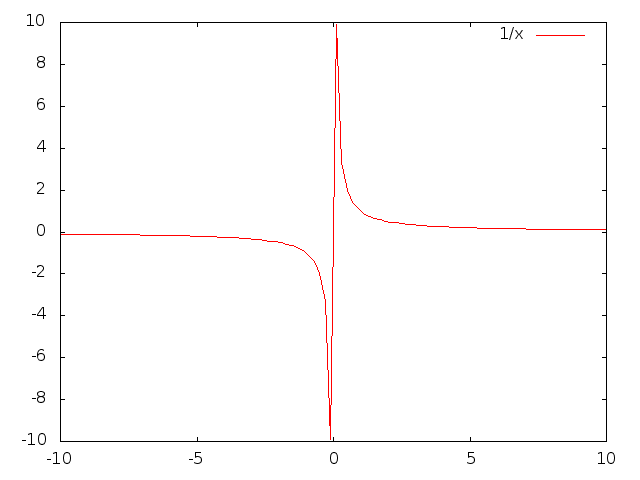
\includegraphics[width=150mm]{1divx.png}

You may plot as many functions as you like, user-defined or built-in.
\begin{verbatim}
gnuplot> f(u)=sin(u)
gnuplot> g(t)=cos(t)
gnuplot> plot f(x),g(x)
gnuplot> plot f(x),g(x),sin(x+pi),cos(x+pi)
\end{verbatim}
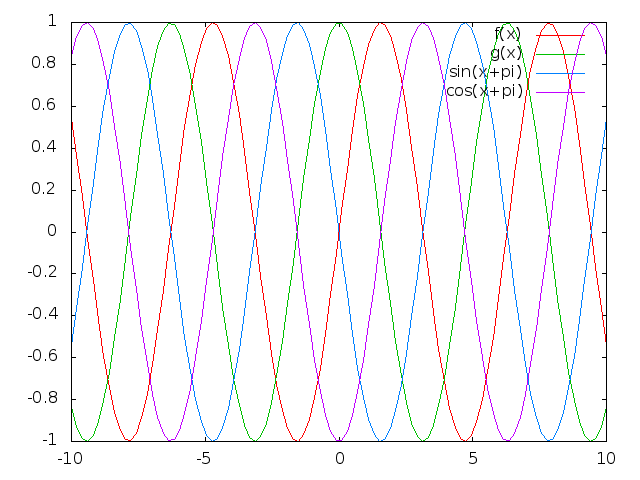
\includegraphics[width=150mm]{multi-plots.png}

I really do mean as many as you like; you are only limited by your patience and the memory of your computer.

\begin{verbatim}
gnuplot> plot sin(x), cos(x), sin(x), cos(x), sin(x), cos(x), sin(x) ...
\end{verbatim}

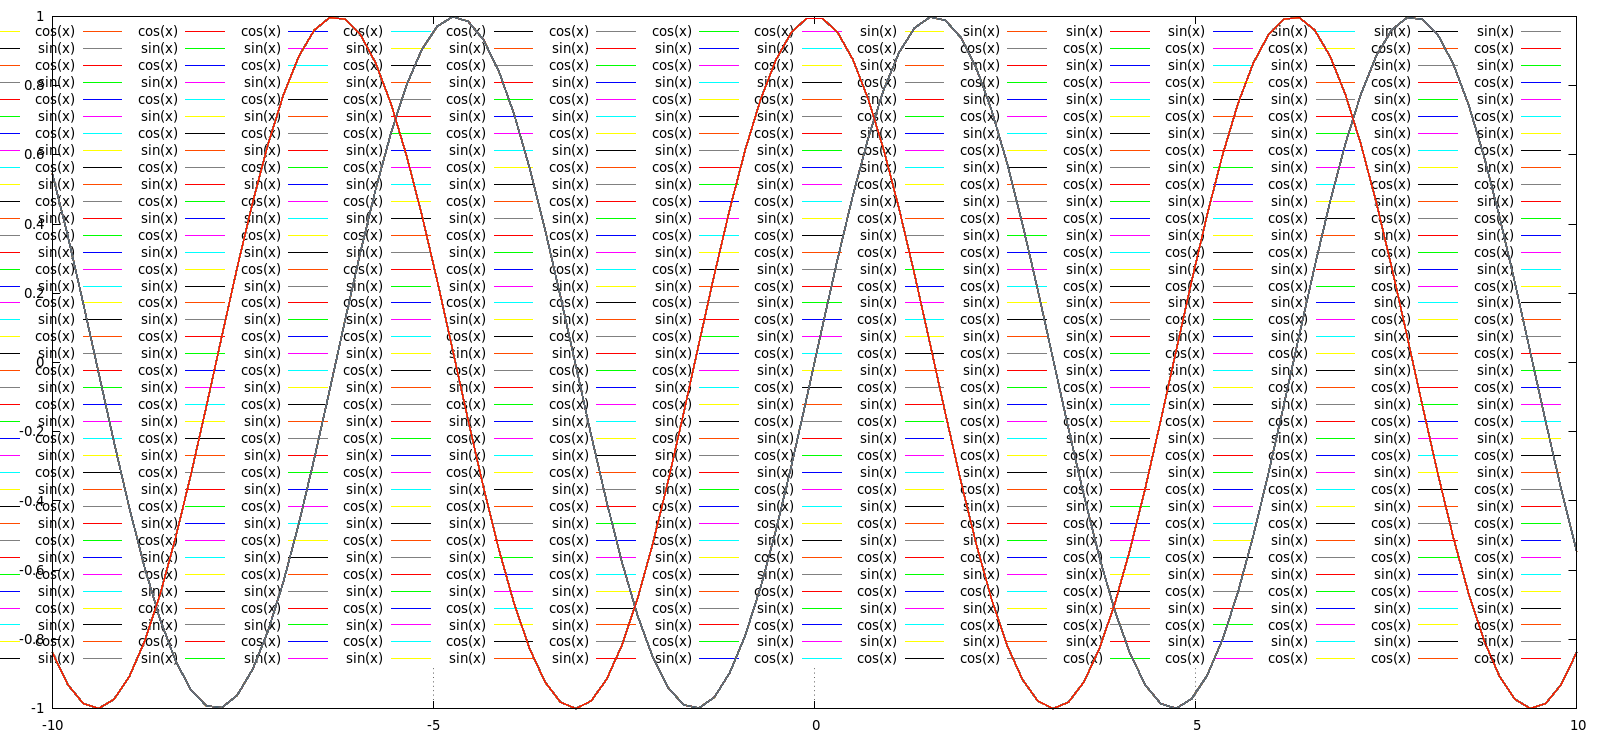
\includegraphics[width=150mm]{too-many-plots.png}

%TODO talk about overlapping lines

You can usually match a function to its graph by the color, but gnuplot also provides different plotting styles.

%TODO Talk about plotting style
%TODO Talk about overlapping plots

You may have noticed that we can use any independent variable we feel like when defining a function, but we always use \verb+x+ when plotting. In fact, if we try to use another variable, we get an error.
\begin{verbatim}
gnuplot> f(t) = t**2
gnuplot> plot f(t)
         undefined variable: t

\end{verbatim}

This is because \verb+x+ and \verb+y+ are special variables gnuplot calls \emph{dummy variables}.

\begin{verbatim}
gnuplot> show dummy

	dummy variables are "x" and "y"

\end{verbatim}

You can change these with \verb+set dummy+. For details, see \verb+ help dummy+.

%TODO talk about what plot does with undefined values

\section{Interactively panning the viewing window}

The default plotting window in gnuplot, \verb+wxt+, has these options for moving around.

\begin{center}
	\begin{tabular}{|c|l|}
	\hline 
	Command & Effect \\
	\hline
	Wheel up & Pan up \\
	\hline
	Wheel up & Pan down \\
	\hline
	Shift + wheel up & Pan left \\
	\hline
	Shift + wheel down & Pan right \\
	\hline
	\end{tabular}
\end{center}



\section{Interactive zooming}

Gnuplot has a good autoscaling algorithm, so many of the plotting options in a TI Calculator are unnecessary. Furthermore, there are many options for using mouse and keyboard in the plotting window. To see them, type \lstinline+h+ while in a plotting window. In the documentation, these are the meanings for various mouse actions:

\begin{center}
	\begin{tabular}{|l|l|}
	\hline 
	\verb+<B1>+ & left click \\
	\hline
	\verb+<B1-Motion>+ & left click and drag \\
	\hline
	\verb+<B2>+ & middle click \\
	\hline
	\verb+<B2-Motion>+ & scroll wheel \\
	\hline
	\verb+<B3>+ & right click \\
	\hline
	\end{tabular}
\end{center}

Here are some of the most useful commands for 2D zooming.

\begin{center}
	\begin{tabular}{|c|l|}
	\hline 
	Command & Meaning \\
	\hline
	Right-click and release & Choose zoom window \\
	\hline
	Ctrl + Scroll up & Zoom in \\
	\hline
	Ctrl + Scroll down & Zoom out \\
	\hline
	\verb+q+ & Exit plot and return to command line \\
	\hline
	\verb+e+ & Replot \\
	\hline
	\verb+a+ & Autoscale \\
	\hline
	\verb+p+ and \verb+n+ & Hop back and forwards to previous and next zoom settings\\
	\hline
	\verb+u+ & Unzoom (reset to original plot settings) \\
	\hline
	\verb+7+ & Cycle through aspect ratios \\
	\hline
	\end{tabular}
\end{center}

Some of the TI auto-zoom functions do transfer to gnuplot; others do not exist as built-in options.

%TODO finish this table
\begin{center}
	\begin{tabular}{|c|c|l|}
	\hline 
	TI calculator & gnuplot command & Meaning \\ 
	\hline 
	\verb+Zbox+ & Right-click  & Select a box with the cursor and zoom to it. \\
	\hline
	\verb+Zoom In+ & Ctrl-Wheel-Up & \\
	\hline
	\verb+Zoom Out+ & Ctrl-Wheel-Down & \\
	\hline
	\verb+Zdecimal+ & No equivalent & \\
	\hline
	\verb+Zsquare+ & \lstinline+set size square+ & \\
	\hline
	\verb+Zstandard+ & \lstinline+set size square+ & \\
	\hline
	\verb+Ztrig+ & \lstinline+set size square+ & \\
	\hline
	\verb+Zinteger+ & \lstinline+set size square+ & \\
	\hline
	\verb+Zinteger+ & \lstinline+set size square+ & \\
	\hline
	\verb+Zinteger+ & \lstinline+set size square+ & \\
	\hline
	\end{tabular}
\end{center}

%TODO talk about what to do if you get stuck or your mouse is not responding, e.g. m toggles mouse

\section{Plotting display tricks}

\begin{center}
	\begin{tabular}{|c|l|}
	\hline 
	Command & Effect \\
	\hline
	Double left-click & Copy coordinates to clip board \\
	\hline
	Command & Meaning \\
	\hline
	Command & Meaning \\
	\hline
	\end{tabular}
\end{center}

\section{Modifying plots using the command line}

Gnuplot was used long before computer mouses were widely available, so while the mouse is indubitably convenient, it is not really necessary; anything that can be done with the mouse can be done with the keyboard.

This is actually quite useful for doing things like dynamics plots and scripting, so it's worth learning even if you don't use it much in practice.

%TODO Talk about xmin, xmax, ymin, ymax, xscl, yscl, xres, yres


\section{Terminals}

\section{Scripting}

\section{Dynamic plots}

\begin{verbatim}
gnuplot> plot 1/0
                 ^
         all points y value undefined!

\end{verbatim}


%TODO Graph styles
%TODO GridOn, GridOff, LabelOn, LabelOff
%TODO Horizontal and vertical lines
%TODO intersections, maxima and minima
%TODO lists, strings, for loops
%TODO reading from a text file

%TODO parametric, polar, sequence,  and stat plots

%TODO random numbers
\begin{verbatim}
nathaniel@nathaniel-laptop:~$ gnuplot -e "print rand(0)"
0.222457440974512
nathaniel@nathaniel-laptop:~$ gnuplot -e "print rand(0)"
0.222457440974512
\end{verbatim}


\chapter{Bibliography}
\begin{verbatim}

gnuplot 4.7
An Interactive Plotting Program
Thomas Williams & Colin Kelley
2012 Version 4.7 (cvs)

Gnuplot in Action
Understanding Data with Graphs
Philipp K. Janert
2010 by Manning Publications Co.

TI-84 Plus and
TI-84 Plus Silver Edition
Guidebook
2004--2010 Texas Instruments Incorporated

\end{verbatim}

\chapter{History of gnuplot and TI graphing calculators}

\end{document}
